\section{Построение репродукционных выборок}

\fixme{ДОПИСАТЬ ПРО РЕПРОДУКЦИЮ ПО ГИСТОГРАММЕ}

Одним из ключевых применений унарной классификации является задача создания синтетических табличных данных, особенно актуальная в условиях ограниченного доступа к реальным данным. Такие ограничения~\cite{gal2023synthetic} могут быть обусловлены законодательными мерами по защите персональных данных~\cite{joshi2024synthetic}, коммерческой тайной или просто недостаточным объёмом исходной выборки. Синтетические данные находят применение в обучении моделей, увеличении объёма обучающих данных~\cite{belyaeva2020synthetic}, обеспечении воспроизводимости научных исследований~\cite{grund2022using} и безопасной передаче информации между организациями.

Основное требование к синтетическим данным -- сохранение статистических и структурных свойств оригинального распределения при гарантии отсутствия утечки чувствительной информации \cite{bauer2024comprehensive}. На практике это означает, что синтетические выборки должны отражать ту же плотность вероятности, что и оригинальные данные, при этом исключая прямое копирование реальных наблюдений.

Для генерации синтетических данных применяются как классические статистические методы, так и модели, основанные на машинном обучении~\cite{figueira2022survey} -- например, вариационные автоэнкодеры (VAE)~\cite{wan2017variational}, генеративно-состязательные сети (GAN)~\cite{jordon2018pate}, диффузионные модели~\cite{villaizan2024diffusion} и др. \cite{akkem2024comprehensive}. Статистические методы обеспечивают согласованность оценок -- то есть, при росте объёма выборки оценка приближается к истинному распределению. В то же время, нейросетевые методы, несмотря на высокую эмпирическую эффективность, зачастую не обладают теоретическими гарантиями сохранения статистических свойств.

В работе \cite{synthetic2025unary} предлагается альтернативный подход к генерации синтетических данных, основанный на унарной классификации. В отличие от традиционных генеративных моделей, которые непосредственно генерируют новые объекты, здесь нейросеть обучается различать реальные точки данных и точки, равномерно сэмплированные из фонового распределения на ограниченной области пространства. В дальнейшем результат классификации используется для фильтрации вновь сгенерированных фоновых точек, формируя репродукционную выборку, приближающую плотность исходных данных.

\subsection{Постановка задачи}

Рассмотрим множество наблюдений \(X = \{x_1, x_2, \dots, x_n\} \in [0, 1]^d\), представляющее собой выборку из неизвестного распределения с плотностью \(f(x)\). Цель состоит в построении синтетической выборки \(\tilde{X} = \{\tilde{x}_1, \tilde{x}_2, \dots, \tilde{x}_m\}\), которая сохраняет статистические свойства оригинального распределения (рисунок~\cref{fig:synthetic_data_task}).

\begin{figure}[ht]
    \centerfloat{
        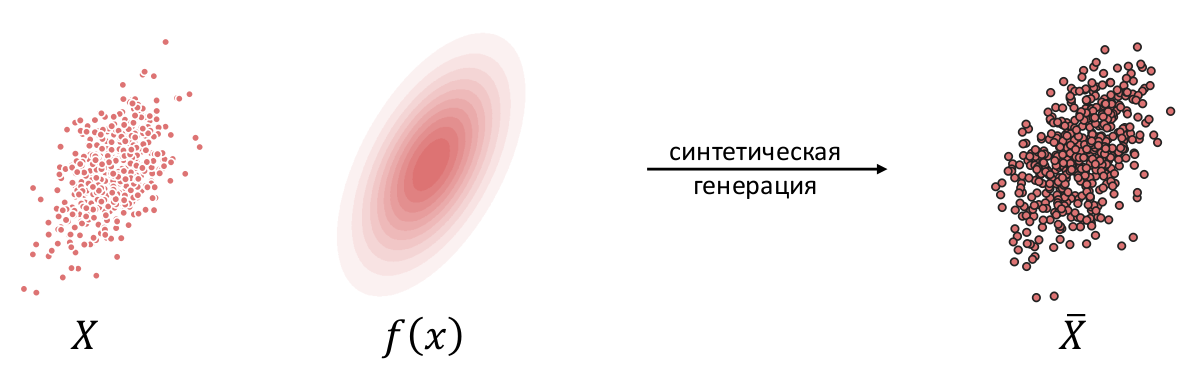
\includegraphics[width=\linewidth]{Dissertation/images/ch3/reproduction/synthetic_data_task.png}
    }
    \caption{Схематичное представление задачи создания синтетических данных}
    \label{fig:synthetic_data_task}
\end{figure}

Традиционные методы оценки плотности распределения обычно предполагают построение непараметрической оценки \(\hat{f}(x)\) для аппроксимации \(f(x)\). В отличие от этого, предлагается альтернативный подход, основанный на унарной классификации, где нейронная сеть обучается различать реальные точки данных и выборки, взятые из равномерного фонового распределения.

\subsection{Обучение классификатора}

В рамках предложенного подхода рассматривается фоновое распределение -- равномерное на компакте \([0, 1]^d\). Из него отбирается множество точек \(B = \{b_1, b_2, \dots, b_n\}\), равное по мощности множеству \(X\).

На объединённой выборке \(X \cup B\) унарно обучается многослойный персептрон \(c_n(x): [0, 1]^d \to [0, 1]\). Метки классов задаются следующим образом:
\[
\left\{
\begin{alignedat}{2}
    &&c_n(x) \rightarrow 1, \quad &\text{если } x \in X, \\
    &&c_n(b) \rightarrow 0, \quad &\text{если } b \in B, \\
\end{alignedat}
\right.
\]

Для обучения модели используется функция потерь среднеквадратичной ошибки (MSE):
\[
L = \sum_{x \in X} (1 - c_n(x))^2 + \sum_{b \in B} (0 - c_n(b))^2.
\]

Выбор MSE вместо кросс-энтропии обусловлен желанием получить гладкую аппроксимацию функции плотности. В отличие от кросс-энтропии, которая стремится к резкому разделению классов, MSE интерпретируется как регрессионная функция, позволяющая трактовать выход сети как сглаженную аппроксимацию плотности без необходимости нормировки.

Особенность метода -- генерация новых фоновых точек на каждом обучающем шаге (эпохе), а не фиксированное множество \(B\), заданное в начале. Это обеспечивает более полное покрытие области и снижает переобучение на конкретных фоновых примерах.

\subsection{Создание репродукционных данных}

После завершения обучения классификатора, синтетические данные получаются путём фильтрации новых фоновых точек. Из равномерного распределения на \([0, 1]^d\) сэмплируется множество \(\tilde{B}\), и каждая точка \(\tilde{b} \in \tilde{B}\) включается в итоговую выборку с вероятностью \(c_n(\tilde{b})\). То есть:
\[
\tilde{X} = \{ \tilde{b} \in \tilde{B} \mid \xi < c_n(\tilde{b}) \}, \quad \xi \sim \text{Uniform}(0,1).
\]

Такой подход позволяет строить выборку, приближенную к оригинальной плотности \( f(x) \), не предполагая явной генеративной модели. При этом плотность оценивается через классификационную задачу, что позволяет интерпретировать модель как адаптивную гистограмму.

\subsection{Экспериментальное исследование}

Для демонстрации эффективности метода проведены эксперименты на модельных датасетах с известной структурой (рисунок~\cref{fig:synthetic_datasets}). Это позволяет объективно оценить способность модели к воспроизведению статистических свойств. Рассматривались следующие выборки:

\begin{itemize}
  \item \textbf{Спираль}: двумерная выборка, где точки образуют спираль. Проверяется способность метода к моделированию нелинейной кластеризации.
  \item \textbf{Два квадрата}: два раздельных кластера квадратной формы. Оценивается сохранение пространственной структуры и разделимости.
  \item \textbf{Нормальное распределение}: двумерное распределение с известными параметрами. Проверяется соответствие ковариационной структуры.
  \item \textbf{Многомерное нормальное распределение}: 10-мерный аналог предыдущего случая, оценивающий качество генерации в высокоразмерном пространстве.
\end{itemize}

\begin{figure}[ht]
    \centerfloat{
        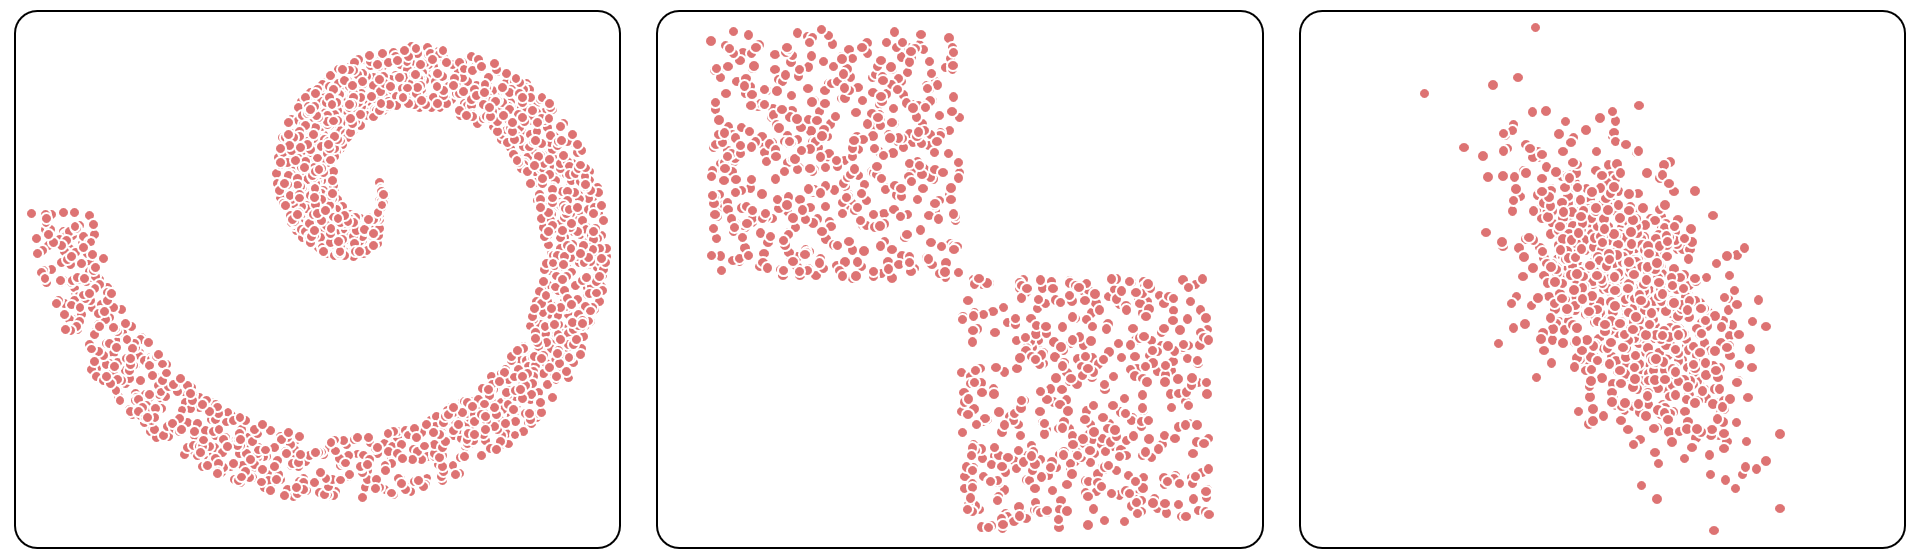
\includegraphics[width=\linewidth]{Dissertation/images/ch3/reproduction/datasets.png}
    }
    \caption{Использованные наборы данных для построения репродукционных выборок (спираль, два квадрата и гауссиан)}
    \label{fig:synthetic_datasets}
\end{figure}

Визуализация результатов (рисунок~\cref{fig:synthetic_results}) демонстрирует, что сгенерированные данные точно воспроизводят форму, плотность и вариативность оригинальных данных. В случае многомерного нормального распределения сохраняется ковариационная структура, хотя наблюдается небольшое увеличение дисперсии -- эффект, обусловленный ростом размерности и разрежённостью пространства.

\begin{figure}[ht]
    \centerfloat{
        \hfill
        \subcaptionbox{Спираль}{%
            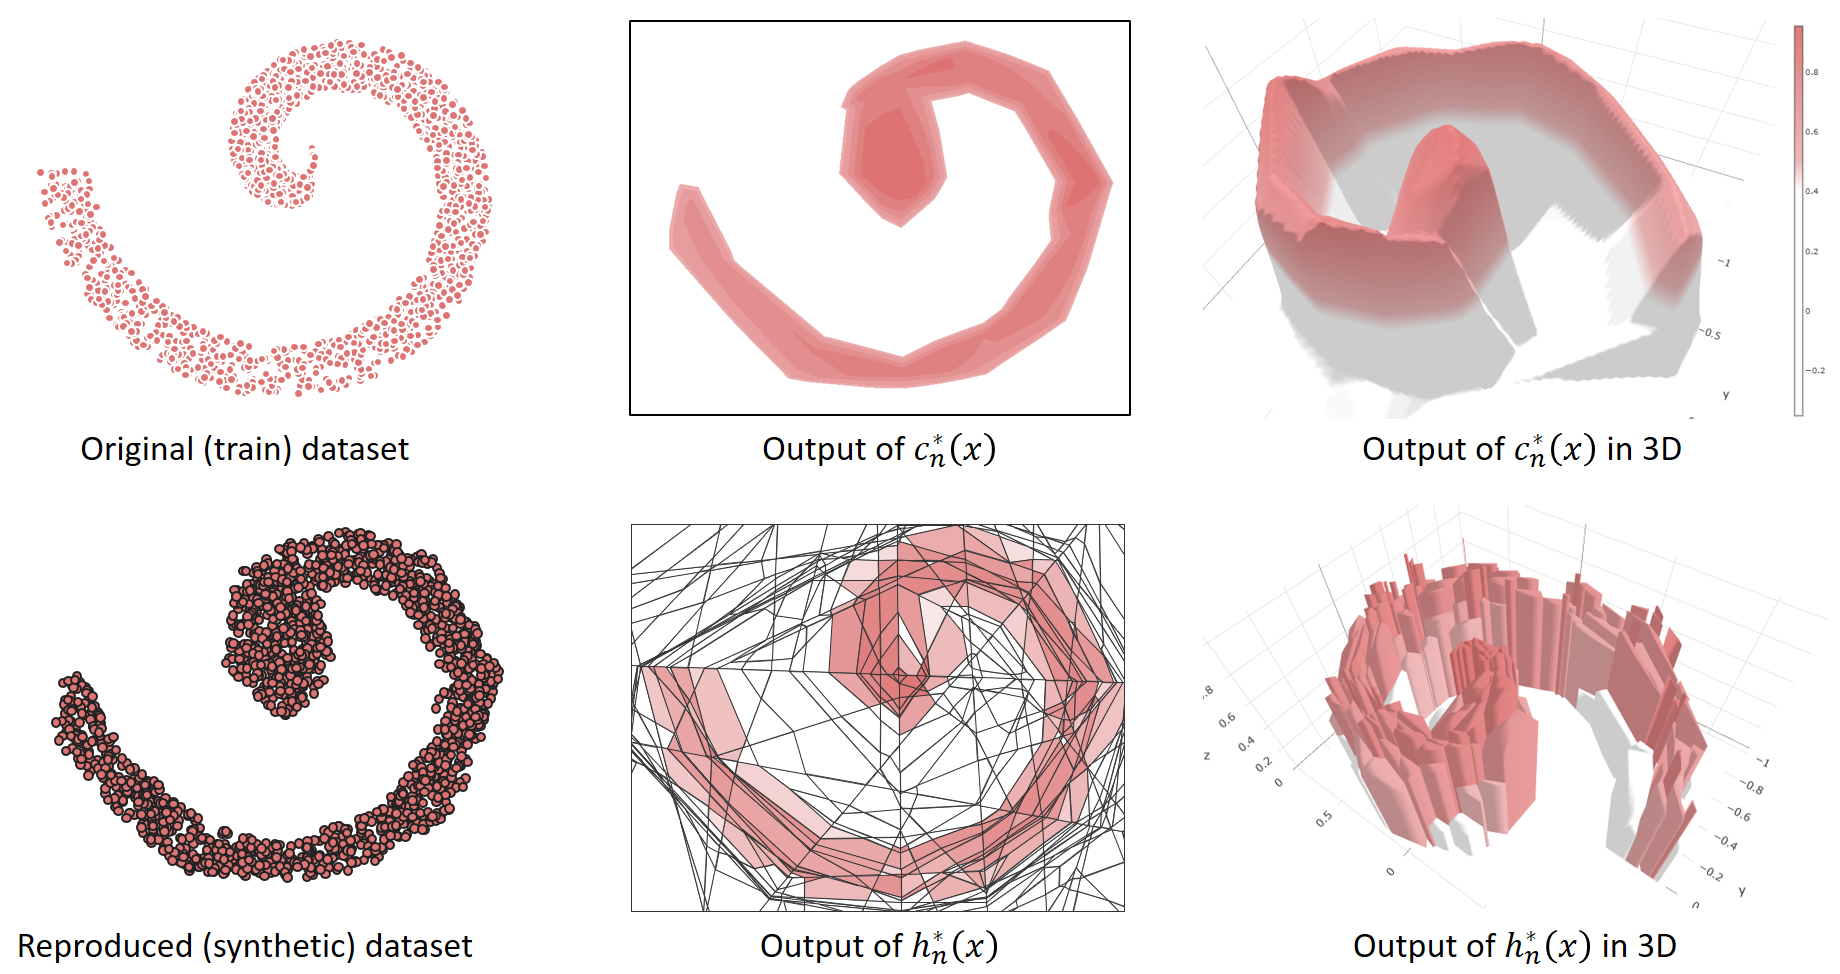
\includegraphics[width=0.32\linewidth]{Dissertation/images/ch3/reproduction/spiral.png}}
        \hfill
        \subcaptionbox{Два квадрата}{%
            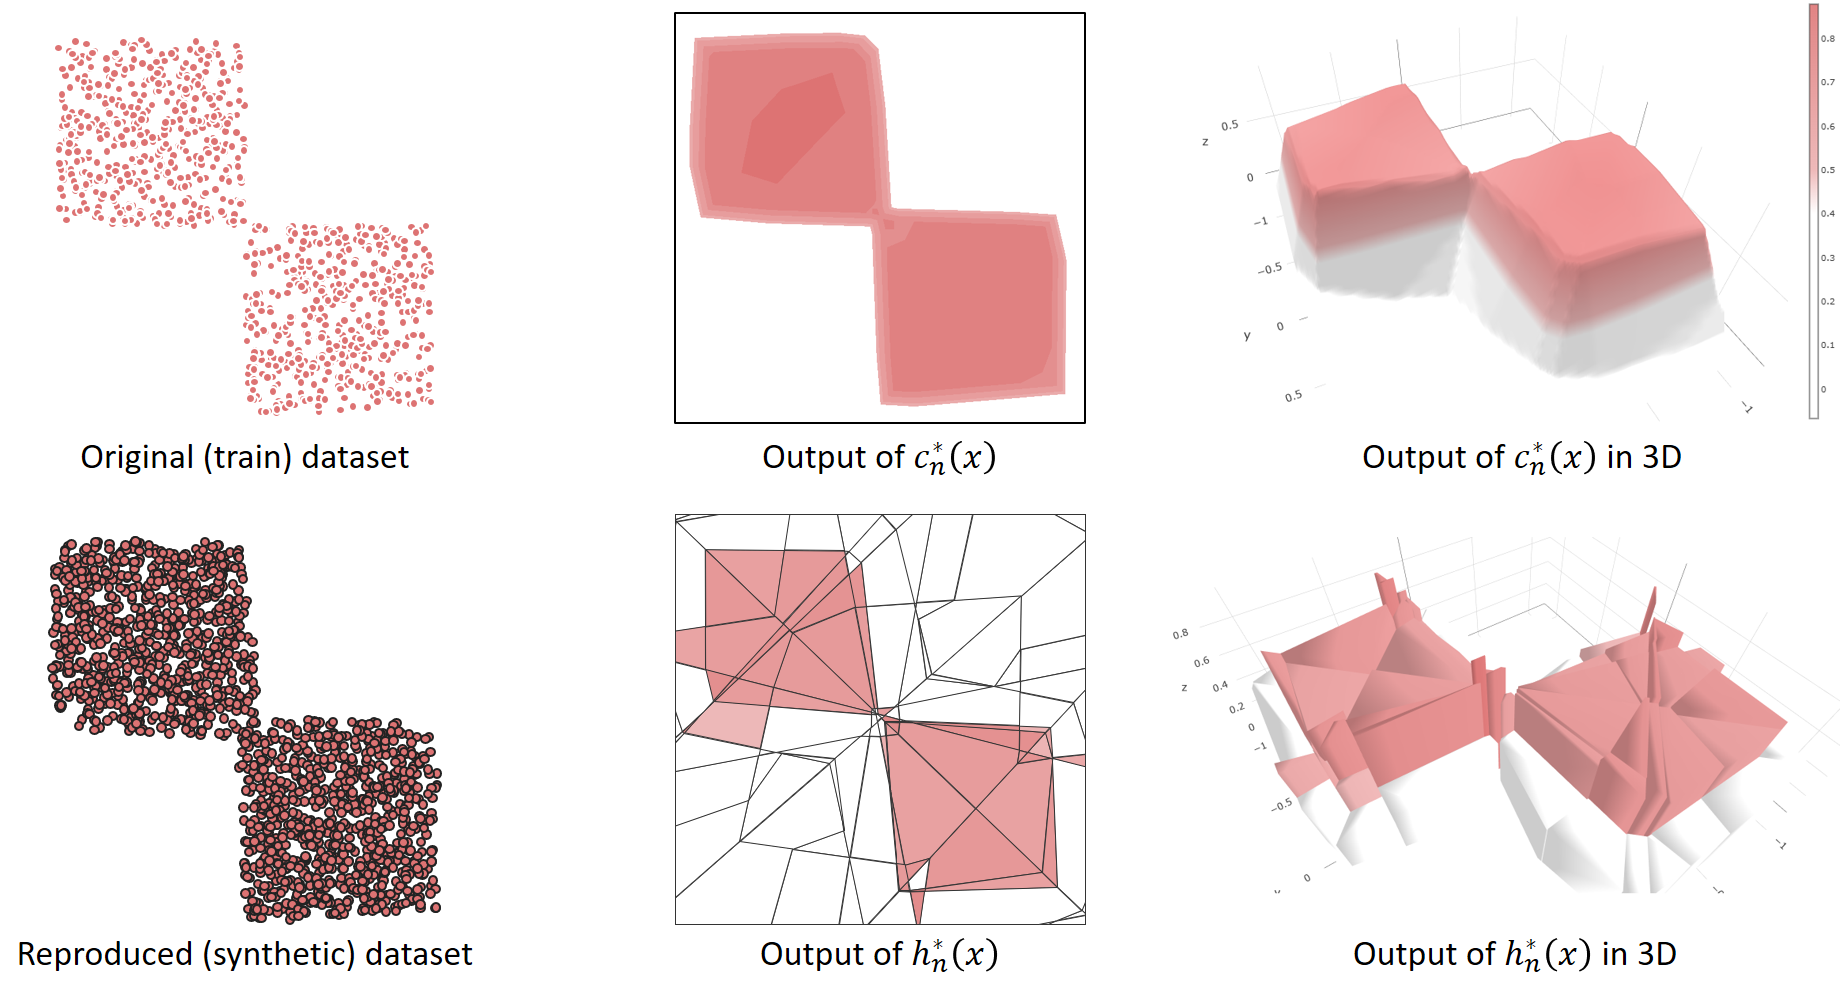
\includegraphics[width=0.32\linewidth]{Dissertation/images/ch3/reproduction/two-square.png}}
        \hfill
        \subcaptionbox{Смесь нормальных распределений}{%
            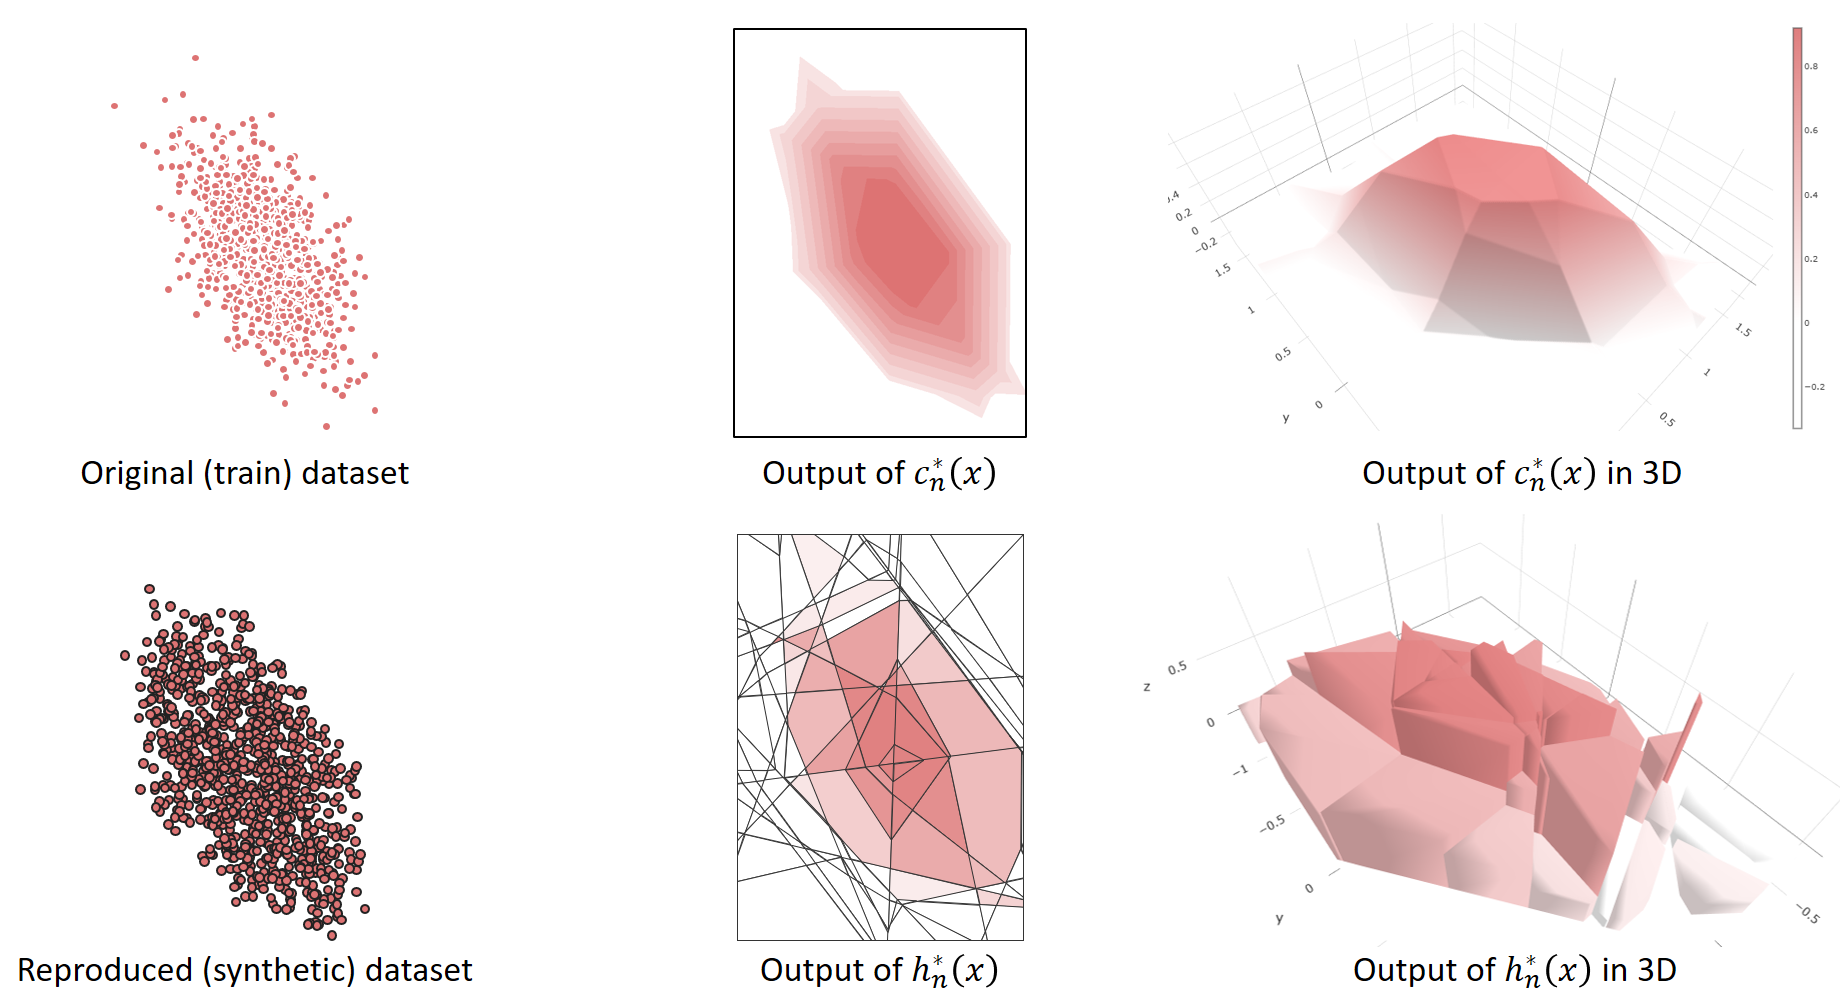
\includegraphics[width=0.32\linewidth]{Dissertation/images/ch3/reproduction/gaussian.png}}
        \hfill
    }
    \caption{результаты эксперимента с синтетическими данными}
    \label{fig:synthetic_results}
\end{figure}

\subsubsection{Архитектура и параметры обучения}

Модель обучалась на 100 эпохах, размер батча -- 32. Использовались различные архитектуры сети:
\begin{itemize}
  \item \textbf{d-10-1}: минималистичная модель с одним скрытым слоем.
  \item \textbf{d-10-100-1}: глубокая архитектура с повышенной ёмкостью.
  \item \textbf{d-10-10-10-1}: сбалансированная конфигурация.
\end{itemize}

Оптимизация осуществлялась методом Adam~\cite{adam2014method} с шагом обучения \(10^{-3}\). Функция активации -- модульная.

\subsubsection{Ограничения}

Преимущество предложенного подхода заключается в естественной аппроксимации плотности через сетевую структуру, эквивалентную адаптивной гистограмме. Однако с ростом размерности пространства наблюдается ухудшение качества генерации из-за разреженности, что требует более сложной архитектуры и дополнительных механизмов фильтрации. Одним из решений является введение более высокого порога уверенности \(\beta\), при котором в синтетическую выборку включаются только точки с \(c(x) > \beta\), снижая шум, но уменьшая разнообразие.

Кроме того, в отличие от генеративных моделей, основанных на латентных переменных (например, CTGAN \cite{habibi2023imbalanced}, TVAE \cite{ishfaq2018tvae}), рассматриваемый метод не требует обучения скрытого представления и обладает более прозрачной интерпретируемостью за счёт прямой связи с оценкой плотности.

Важно отметить, что модель может наследовать структурные и социальные смещения из обучающих данных. Поэтому при генерации синтетических выборок, особенно в задачах с социально значимой информацией, требуется дополнительный контроль справедливости.

\subsubsection{Выводы}

Таким образом, метод построения репродукционных выборок через унарную классификацию представляет собой эффективную альтернативу генеративным моделям. Он сочетает в себе простоту реализации, теоретическую интерпретируемость и способность воспроизводить сложные структуры данных. Это делает его перспективным инструментом для синтетической генерации данных, особенно в условиях ограниченного доступа к реальным выборкам.
